\documentclass[11pt,reqno,final]{amsart}

\pdfcompresslevel=0
\pdfobjcompresslevel=0

\usepackage[dvipsnames]{xcolor}% adds colors
\usepackage{amsmath, amsthm}% {amsfonts, amssymb}

% New Characters
\usepackage[latin1]{inputenc}%
\usepackage[T1]{fontenc}

\usepackage{MnSymbol}
\usepackage[normalem]{ulem}% underlining

\usepackage[theoremfont, largesc]{newpxtext} % different text,math font
\usepackage{newpxmath}

\makeatletter
\DeclareMathRadical{\sqrtsign}{symbols}{112}{largesymbols}{112}
% \let\sqrt=\undefined
% \DeclareRobustCommand\sqrt{\@ifnextchar[\@sqrt{\mathpalette\@x@sqrt}]}
% \def\@x@sqrt#1#2{%
%  \setbox\z@\hbox{$\m@th#1\sqrtsign{\mkern1mu #2}$}
%  \mkern3mu\box\z@}
\makeatother




% Page Typesetting
\usepackage[final]{microtype}
\usepackage{relsize}
\usepackage[margin=1in]{geometry}
\usepackage{framed}
\usepackage{tikz}
\usepackage{setspace}

\usepackage{hyperref}
\hypersetup{
  final,
  pdftitle={Math 135 - Definition of the Derivative},
  pdfauthor={Bonventre}, 
  linktoc=page,
  pagebackref,
  colorlinks=true,
  citecolor=PineGreen,
  linkcolor=PineGreen,
  linkbordercolor=PineGreen,
}


% Internal References

\usepackage[inline,shortlabels]{enumitem}

% \numberwithin{equation}{section} 
\numberwithin{figure}{section}

\usepackage[nameinlink,capitalise,noabbrev]{cleveref}

\crefname{equation}{}{} % get \cref to behave as \eqref

% \theoremstyle{plain} % bold name, italic text
\newtheorem{theorem}[equation]{Theorem}%
\newtheorem*{theorem*}{Theorem}%
\newtheorem{lemma}[equation]{Lemma}%
\newtheorem{proposition}[equation]{Proposition}%
\newtheorem{corollary}[equation]{Corollary}%
\newtheorem{conjecture}[equation]{Conjecture}%
\newtheorem*{conjecture*}{Conjecture}%
\newtheorem{claim}[equation]{Claim}%
\newtheorem{question}{Question}

\theoremstyle{definition} % bold name, plain text
\newtheorem{definition}[equation]{Definition}%
\newtheorem*{definition*}{Definition}%
\newtheorem{example}[equation]{Example}%
\newtheorem*{example*}{Example}%
\newtheorem{remark}[equation]{Remark}%
\newtheorem{notation}[equation]{Notation}%
\newtheorem{convention}[equation]{Convention}%
\newtheorem{assumption}[equation]{Assumption}%
\newtheorem{exercise}[question]{Exercise}

% ---------- macros
\newcommand{\set}[1]{\left\{#1\right\}}%
\newcommand{\sets}[2]{\left\{ #1 \;|\; #2\right\}}%
\newcommand{\longto}{\longrightarrow}%
\newcommand{\into}{\hookrightarrow}%
\newcommand{\onto}{\twoheadrightarrow}%

\usepackage{harpoon}
\newcommand{\vect}[1]{\text{\overrightharp{\ensuremath{#1}}}}

\newcommand{\del}{\partial}%

\newcommand{\ki}{\chi}
\newcommand{\ksi}{\xi}
\newcommand{\Ksi}{\Xi}

\newcommand{\dlim}{\displaystyle\lim}

% %%%%%%%%%%%%%%%%%%%%%%%%%%%%%%%%%%%%%%%%%%%%%%%%%%%%%%%%%%%%%%%%%%%%%%%%%%%%%%%%%%%%%%%%%%%%%%%%%%%%

\begin{document}
\onehalfspacing

\begin{center}
        \textbf{\Large Math 135, Calculus 1, Fall 2020}\\[10pt]
        {\large 10-05: Definition of the Derivative (Section 3.1)}
\end{center}

\thispagestyle{empty}

\renewcommand{\thesection}{\Alph{section}}

% \vspace{-1pt}

This section introduces the \textbf{derivative}, one of the most important concepts in all of mathematics and science.  
It is the foundation of calculus.  

\subsection*{What is the derivative?}

We have already seen examples of the derivative in our earlier work:
the derivative of $f(x)$ is
\begin{itemize}
\item the \textbf{slope} of the tangent line to the graph of the function $f(x)$, or
\item the \textbf{instantaneous velocity} of $f(x)$ at a point.
\end{itemize}

We compute this by taking the limit of the average velocities/slopes of secant lines:
if we fix one endpoint $x = a$, then 
\[
        \mbox{average velocity on the interval $[a,x]$} = \mbox{slope of the secant line over $[a,x]$}
        = \dfrac{\Delta y}{\Delta x}
        = \dfrac{f(x) - f(a)}{x-a}        
\]

Taking the limit, we get the following:
\begin{definition*}
        The \textbf{derivative} of $f(x)$ at the point $x = a$, denoted by $f'(a)$ (read as ``f prime of a''), is given by
        \begin{framed}
                \begin{equation}
                        \label{DEFDER_EQ}
                        f'(a) = \dlim_{x \to a}\dfrac{f(x) - f(a)}{x-a}.
                \end{equation}
        \end{framed}
        \renewcommand{\arraystretch}{0.5}
        This limit may or may not exist.  If the limit exists, we say that
        the function is {\bf differentiable} at $x = a$.       
\end{definition*}

The fraction in Equation \cref{DEFDER_EQ} is called the \textbf{difference quotient}.
If we evaluate the difference quotient at $x = a$ we get $\mathbf{\frac{0}{0}}$,
a familiar indeterminant form that can be ANYTHING.
So we must simplify the difference quotient in order to evaluate the limit.

\begin{exercise}
        Use Equation \cref{DEFDER_EQ} to compute the derivative of $f(x) = x^2 - 3x$ at the point $x = 1$.
        In other words, compute $f'(1)$.  What is the equation of the tangent line to $f$ at $x = 1$?\\
        \textit{Hint: What is the value of $a$? What is $f(a)$? Can we factor the numerator?}\\
        \textsc{Be careful with your parentheses!}       
\end{exercise}

\newpage

Compare your answer to the above with the following graph of $y = x^2 - 3x$ with the tangent line at $x = 1$.
\begin{center}
        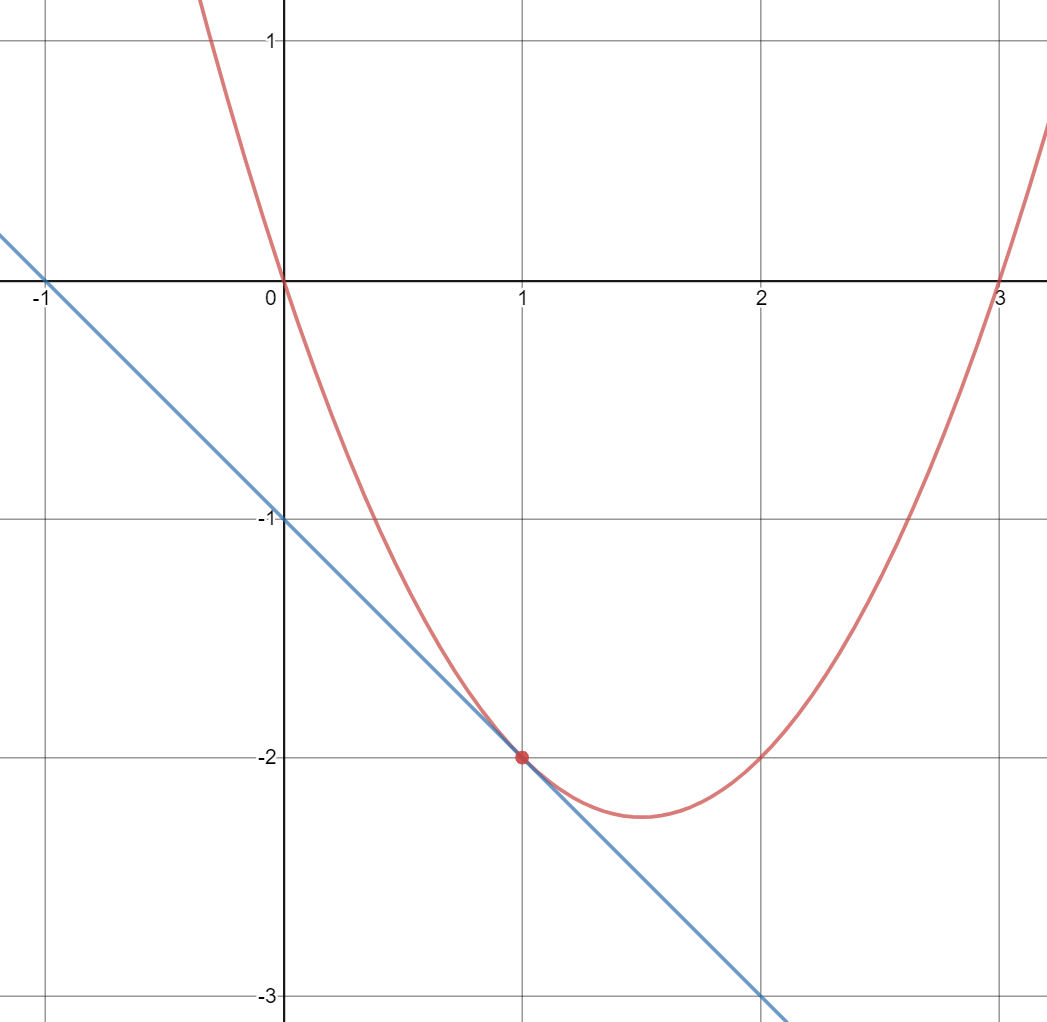
\includegraphics[width=2.5in]{10-05P_tan.png}
\end{center}

We can rewrite the definition from Equation \cref{DEFDER_EQ} by making the substitution $h = x-a$.
Then we have the average velocity on the interval $[a,x] = [a,a+h]$ is the difference quotient
\[
        \dfrac{f(x) - f(a)}{x-a} = \dfrac{f(a+h) - f(a)}{h}.
\]
This has a simpler denominator, but a more complicated numerator.
Since $h \to 0$ as $x \to a$, we have a second definition of the derivative:
\begin{framed}
        \begin{equation}
                \label{DEFDER2_EQ}
                f'(a) = \dlim_{h \to 0}\dfrac{f(a+h) - f(a)}{h}.
        \end{equation}
\end{framed}

$ $

\begin{exercise}
        Use Equation \cref{DEFDER2_EQ} to compute $f'(1)$ for $f(x) = x^2-3x$.
        Confirm that you obtain the same ansqewr as in Exercise 1.\\
        \textit{Hint: What is the value of $a$? What is $f(a+h)$? Can we factor the numerator?}\\
        \textsc{Be careful with your parentheses!}       
\end{exercise}

\newpage

\begin{exercise}
        Consider the function $f(x) = -4x +7$.
        What do you expect for the value of $f'(3)$? Why?
        Confirm your guess using either Equation \cref{DEFDER_EQ} or \cref{DEFDER2_EQ}.
        \vfill
\end{exercise}

\begin{exercise}
        Using either Equation \cref{DEFDER_EQ} or \cref{DEFDER2_EQ},
        find the slope of the tangent line to the function $f(x) = \dfrac{2}{x}+1$ at the point $x = 2$.\\
        \textit{Hint: Can we write the numerator as a single fraction?}
        \vfill
\end{exercise}

\begin{exercise}
        Let $f(x) = \sqrt{x}$. Compute $f'(4)$ using either Equation \cref{DEFDER_EQ} or \cref{DEFDER2_EQ}.\\
        \textit{Hint: Multiply the top and bottom of the difference quotient by the conjugate of the numerator.}
        \vfill
\end{exercise}

\end{document}
